\documentclass{article}

\usepackage{graphicx}
\usepackage{latexsym}

\setlength{\pdfpagewidth}{8.5truein}
\setlength{\pdfpageheight}{11truein}

\def\s{\hbox{s}}
\def\m{\hbox{m}}

\usepackage{fullpage}

\addtolength{\topmargin}{-.5in}
\textheight 9in

\begin{document}

\title{Physics and Math of Music --- Day 3 --- Strings}
\date{Thursday, February 7, 2002}
\author{Peter Folk ({\tt pfolk@uni}) and Paul Grayson ({\tt pgrayson@uni})}
\maketitle

\section*{Strings are oscillators}
So far we have only seen one example of an oscillator, the pendulum.
Today you will learn about another way to make an oscillator --- with
a string.  Oscillators made out of strings work just like pendulums,
so we can do all the same things with them.  However, there {\sl is\/}
one difference:

\section*{Strings have {\it harmonics}}
An oscillator has one natural frequency, and will not vibrate at any
other.  A string, however, can vibrate in many different ways.  Here
are some of them:
\begin{figure}[h]
\begin{center}
	\input figures/string_harmonics.tex
	\caption{Different harmonics of a vibrating string}
\end{center}
\end{figure}
The second vibration has twice the frequency of the first; the third
has three times the frequency, and so on.  See if you can make all of
these using a slinky as your string!  Next time you are talking on the
phone, try this with the phone cord!  How many harmonics {\sl can\/}
you make?

Since strings can oscillate at many different frequencies, it is a
good idea to think of them as many different oscillators put together
--- just like our ruler with many pendulums.

\section*{We can calculate the frequencies of a string}
We can calculate the natural frequencies of a string, using a
formula very similar to the one for pendulums.  This time, however, the
frequencies depends not just on the length $L$, but also on the mass
of the string $m$ and the tension $T$ (the force you are pulling with
to stretch it out):
$$ f = 
 1\cdot{1 \over 2} \sqrt{T \over m L}\,\,\,\hbox{, }\,\,\,
 2\cdot{1 \over 2} \sqrt{T \over m L}\,\,\,\hbox{, }\,\,\,
 3\cdot{1 \over 2} \sqrt{T \over m L}\,\,\,\hbox{, ...}
$$
The most important thing here is that $1$, $2$, $3$, ... relationship.
Compare this to the pendulum formula and notice that there is a square
root with some kind of force in the numerator and some kind of length
in the denominator in both formulas!

\section*{Strings can resonate too}
Just like a pendulum, a string can resonate.  If you push it with a
frequency near any one of the natural frequencies, it will start
vibrating at that frequency.  If you send in a wave made up of two
frequencies near two different natural frequencies of the string, what
do you think will happen? (Hint: remember what happens when two people
blow on two pendulums at their two natural frequencies!)

\section*{From yesterday: make any wave out of sine waves}
Here's a picture (which I stole) that shows how you can make a square
wave by adding a bunch of sine waves together:

\begin{figure}[h]
\begin{center}
	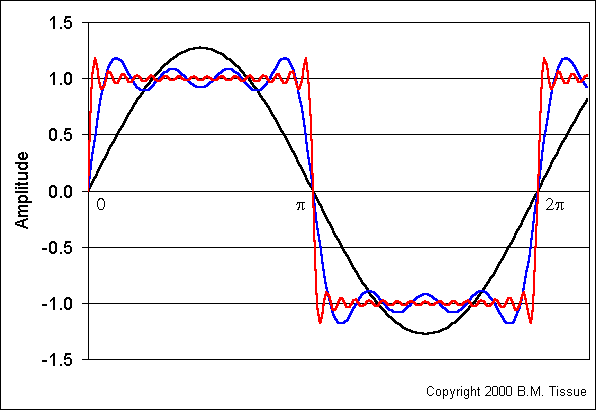
\includegraphics[width=4in]{figures/square_wave.png}
	\caption{One, four, and sixteen sine waves added together to
	approximate a square wave.  It takes a lot of sine waves, but
	it can be done!}
\end{center}
\end{figure}

\end{document}
